\documentclass{article}[11pt]
\usepackage[frenchb,english]{babel}
\usepackage[T1]{fontenc}
\usepackage[utf8]{inputenc}
\usepackage{amsmath,amssymb,latexsym}
\usepackage{times}
\usepackage{float}
\usepackage[left=2cm,right=2cm,top=2cm,bottom=2cm]{geometry}
\frenchbsetup{StandardLists=true} % � inclure si on utilise \usepackage[french]{babel}
\usepackage{enumitem}
\usepackage{fancyhdr}
\usepackage{mathrsfs}
\usepackage{graphicx}
%\usepackage[Algorithme]{algorithm}
%\usepackage{algorithmic}
\usepackage{tikz}
\usepackage{tabularx}
\usetikzlibrary{shapes}
\pagestyle{fancy}
\newcommand{\tr}[1]{{\vphantom{#1}}^{\mathit t}{#1}} 
\renewcommand\headrulewidth{1pt}
\fancyhead[L]{Cours 1�re S}
\fancyhead[R]{Yoann Pietri}
\newcounter{theoremecounter}[subsection]
\usepackage{titlesec}
\setcounter{secnumdepth}{3}% enl�ve la num�rotation apr�s les sections
%\renewcommand\thechapter {\Roman{chapter}}

 \setlength{\parindent}{0pt}

\newcommand{\R}{\mathbb{R}}
\newcommand{\N}{\mathbb{N}}
\newcommand{\Q}{\mathbb{Q}}
\newcommand{\Z}{\mathbb{Z}}
\newcommand{\C}{\mathbb{C}}
\newcommand{\K}{\mathbb{K}}
\newcommand{\eqi}{\Leftrightarrow}
\titleformat{\subsubsection}
   {\normalfont\fontsize{11pt}{13pt}\selectfont\bfseries}% apparence commune au titre et au num�ro
   {\thesubsubsection}% apparence du num�ro
   {1em}% espacement num�ro/texte
   {}% apparence du titre

\tikzstyle{theobox} = [draw=black, very thick,
    rectangle, rounded corners, inner sep=10pt, inner ysep=20pt]
\tikzstyle{theotitle} =[fill=white, text=black,rounded corners,draw=black,very thick]

\fancyhead[L]{Contrôle chapitre 7}

\usepackage[c]{esvect}
\newcommand{\covec}[2]{\begin{pmatrix}#1 \\#2 \end{pmatrix}}

\begin{document}
\center
\Large Contrôle de cours
\flushleft
\center
Produit scalaire
\flushleft \normalsize
Durée du contrôle : 1h10\newline
Ce sujet comporte 3 pages\newline
La calculatrice est autorisée
\subsection*{Exercice 1 (R.O.C., temps conseillé : 10 min) : }
Rappeler les 4 formules donnant le produit scalaire de deux vecteurs du plan en prouvant seulement celle avec les normes\newline

Calculer 
$$\covec{2}{3} \cdot \covec{4}{-5}$$
\subsection*{Exercice 2 (Etude de l'orthogonal, temps conseillé : 25 min) : }
\begin{enumerate}
\item Montrer la caractérisation suivante : 
$$\vv{u} \text{ et } \vv{v} \text{ colinéaires} \Leftrightarrow \vv{u} \cdot \vv{v} = \pm ||\vv{u}|| \times ||\vv{v}||$$
\item Rappeler la définition de 2 vecteurs orthogonaux
\item Soit $\vv{u} \covec{x}{y}$ un vecteur du plan. On note $\{\vv{u}\}^\perp$ l'ensemble des vecteurs orthogonaux à $\vv{u}$. Que vaut $\{\vv{0}\}^\perp$ ? A partir de maintenant, on suppose $\vv{u} \neq \vv{0}$. On veut alors montrer le résultat suivant : tous les vecteurs de $\{\vv{u}\}^\perp$ sont colinéaires entre eux
\item Montrer que $\vv{u} \notin \{\vv{u}\}^\perp$
\item Montrer que $\vv{0} \in \{\vv{u}\}^\perp$
\item Soit $\vv{v} \in \{\vv{u}\}^\perp$. Montrer alors que pour tout $\lambda \in \R$, $\lambda \vv{v} \in \{\vv{u}\}^\perp$
\item On suppose que $x=0$ ($\vv{u} = \covec{0}{y}$). Montrer alors que si $\covec{a}{b} \in \{\vv{u}\}^\perp$ alors $b = 0$. En déduire que tout vecteur de $\{\vv{u}\}^\perp$ s'écrit $\lambda \covec{1}{0}$ et que par conséquent, tous les vecteurs de $\{\vv{u}\}^\perp$ sont colinéaires entre eux. On admet que si l'on suppose $y=0$ et $x\neq 0$, on obtient le même résultat
\item Ainsi, on suppose maintenant $x\neq 0$ et $y \neq 0$. Soient $\vv{v_1}\covec{x_1}{y_1}$ et $\vv{v_2}\covec{x_2}{y_2}$ deux vecteurs de $\{\vv{u}\}^\perp$. Montrer alors 
$$\boxed{y_1 = -\frac{x}{y}x_1} \quad (1)$$
$$\boxed{y_2 = -\frac{x}{y}x_2} \quad (2)$$
\item Montrer alors que 
$$x_1^2y_2^2 + y_1^2x_2^2 = 2x_1y_1x_2y_2$$
\emph{(Indication : on pourra remplacer les $y_1^2$ et $y_2^2$ grâce aux expressions (1) et (2) puis après avoir des simplifications, faites réapparaître des $y_1$ et $y_2$ avec (1) et (2))}
\item Comparer littéralement $\vv{v_1} \cdot \vv{v_2}$ et $||\vv{v_1}|| \times ||\vv{v_2}||$
\item Conclure grace à la question 1
\end{enumerate}
\subsection*{Exercice 3 (Equation cartésienne de sphère, temps conseillé : 15 min) : }
On introduit les points et vecteurs de l'espace. On repère un point de l'espace par 3 coordonnées : $M(x_M,y_M,z_M)$
\center
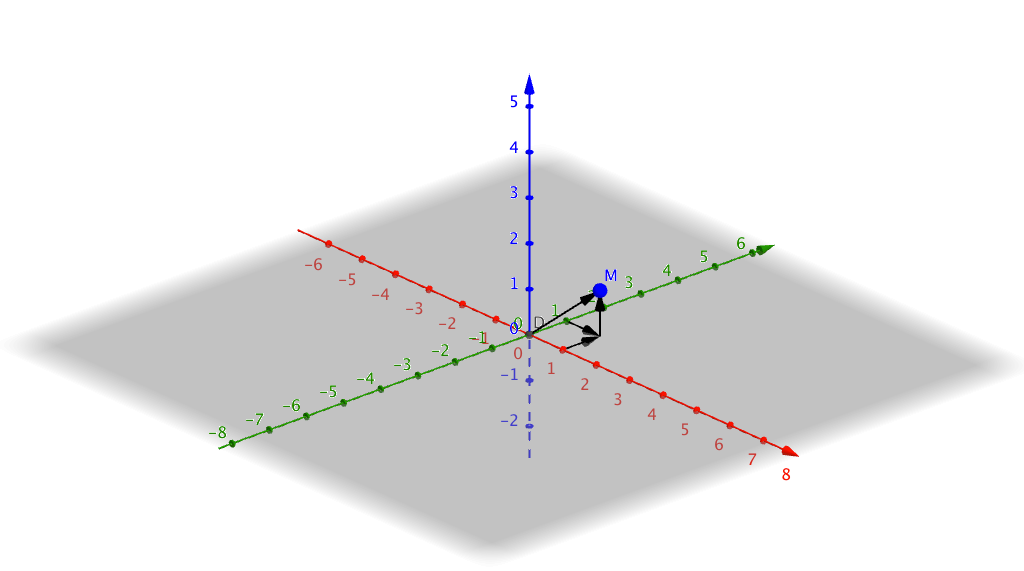
\includegraphics[scale=0.5]{chap7_ill.png}
\flushleft
De même un vecteur $\vv{u}$ de l'espace est repéré par 3 coordonnées : $$\vv{u} \begin{pmatrix} x \\ y \\ z\end{pmatrix}$$
On a toujours $$\vv{AB} \begin{pmatrix} x_B-x_A \\ y_B-y_A \\ z_B-z_A\end{pmatrix}$$
De plus, on définit le produit scalaire
$$\begin{pmatrix} x \\ y \\ z\end{pmatrix} \cdot \begin{pmatrix} x' \\ y' \\ z'\end{pmatrix} = xx' + yy' + zz'$$
et on définit $$||\vv{u}|| = \sqrt{\vv{u}\cdot \vv{u}}$$
\begin{enumerate}
\item Soit $\vv{u} \begin{pmatrix} x \\ y \\ z\end{pmatrix}$. Etablir la formule donnant $||\vv{u}||$ en fonction de $x,y,z$
\item Soit $\mathscr{S}$ la sphère de centre $\Omega(x_\Omega,y_\Omega,z_\Omega)$ et de rayon $r\geq 0$ \emph{(On rappelle qu'une sphère est l'ensemble des points à une distance $r$ de $\Omega$ où la distance entre $\Omega$ et $M$ est donnée par $||\vv{\Omega M}||$)}\newline

 Etablir l'équation cartésienne de cette sphère
\end{enumerate}
\subsection*{Exercice 4 (Théorèmes de Pythagore et d'Al-Kachi, temps conseillé : 15 min) : }
Dans cet exercice, on prouve le fameux théorème de Pythagore puis le (moins fameux) théorème d'Al-Kachi
\begin{enumerate}
\item On considère un triangle rectangle $ABC$ rectangle en $A$ : \newline
\begin{tikzpicture}
\draw (0,0) -- (5,0) -- (0,3) -- (0,0);
\node at (0,0) [left] {$A$};
\node at (0,3) [above] {$B$};
\node at (5,0) [right] {$C$};
\end{tikzpicture}\newline 
Quelle est la valeur de l'angle formé par les vecteurs $\vv{AC}$ et $\vv{AB}$. Quel est son cosinus ?
\item En calculant le produit scalaire $\vv{AC} \cdot \vv{AB}$ avec la méthode des normes et avec celle du cosinus, montrer le fameux théorème de Pythagore
\item On généralise ce résultat avec le théorème d'Al-Kachi : on considère un triangle quelconque 
\begin{tikzpicture}
\draw (0,0) -- (5,0) -- (1,3) -- (0,0);
\node at (0,0) [left] {$A$};
\node at (1,3) [above] {$B$};
\node at (5,0) [right] {$C$};
\end{tikzpicture}\newline 
L'angle formé par les vecteurs $\vv{AC}$ et $\vv{AB}$ est noté $\alpha$. En utilisant une méthode analogue à la question précédente, montrer que 
$$BC^2 = AB^2 + AC^2 - 2 \times AB \times AC \times \cos(\alpha)$$
\end{enumerate}
$$\star \star \star$$
\center
FIN DU SUJET
\end{document}